\documentclass{beamer}

\usepackage[utf8]{inputenc}
\usepackage[ngerman]{babel}
\usepackage[T1]{fontenc}

\usepackage{amsmath,amssymb,amsfonts,amsthm,mathtools}

\usepackage{paralist}
\usepackage{bm}
\usepackage{bbm}
\usepackage{algorithm}
\usepackage{algorithmic}
\usepackage{tikz}
\usepackage{colortbl}

\mode<presentation>
{
  \setbeamertemplate{navigation symbols}{}
    \usetheme{Hannover}
   \setbeamercovered{transparent}
   \useoutertheme{infolines}
}

%\usecaptiontemplate{
%\tiny
%\structure{\insertcaptionname~\insertcaptionnumber:}
%\insertcaption
%}

\title[Simulation einer Populationsdynamik] % (optional, nur bei langen Titeln noetig)
{Simulation einer stochastischen Populationsdynamik}
\subtitle{Vortrag zum Begleitseminars der Bachelorarbeit}
\author[B.Prochnau] % (optional, nur bei vielen Autoren)
{Boris Prochnau}
\institute[Universität Bonn]{Institut für Angewandte Mathematik\\Universität Bonn}

\date {\today}
\setbeamercovered{invisible}

\begin{document}
%
% ****************************************************************************************************
%					preliminaries
% ****************************************************************************************************
%

\begin{frame}
  \titlepage
\end{frame}
\begin{frame}
  \frametitle{Übersicht}
  \tableofcontents
\end{frame}
\section{Einleitung}
\begin{frame}
	\frametitle{Was wird simuliert?}
	\begin{minipage}{0.49\textwidth}
		\begin{figure}
		\centering
		\includegraphics[width=1\linewidth]<1,2,3>{./Lizenzbilder/Zelle1}%	
		\includegraphics[width=1\linewidth]<4>{./Lizenzbilder/Okosystem1}%		
		\end{figure}
	\end{minipage}	
	\begin{minipage}{0.49\textwidth}
		\begin{itemize}
			\item Ein Beute-Beute System mit asexueller Fortpflanzung.\pause
			\item Die Populationsgr"o"se.\pause
			\item[] Die Populationsdynamik.\pause
			\item Ein abgeschlossenes System.
		\end{itemize}
	\end{minipage}
\end{frame}
\begin{frame}
	\frametitle{Dynamik durch Wechselwirkung}\pause
	\begin{minipage}{0.49\textwidth}
		\begin{figure}
		\centering		
		\includegraphics[width=1\linewidth]<2>{./Lizenzbilder/Tier2}%
		\includegraphics[width=1\linewidth]<3>{./Lizenzbilder/Lebensraum1}%
		\includegraphics[width=1\linewidth]<4>{./Lizenzbilder/Pilz2}%
		\end{figure}
	\end{minipage}
	\begin{minipage}{0.49\textwidth}
		\begin{itemize}		
			\item Z.B. durch unabhängige Nahrungsquellen,\pause
			\item Kampf um Lebensraum,\pause
			\item oder dominantes Ressourcenverhalten.
		\end{itemize}
	\end{minipage}
\end{frame}	
	
\section{Modell}
\begin{frame}
	\frametitle{Was beschreibt also unser Modell?}
	\begin{itemize}	
		\item Individuen durch ihre Merkmale, $ x \in X $.
		\item Intrinsische und extrinsische Geburten.\pause
		\item Natürliche Tode und solche, die durch Wettbewerb zu anderen Individuen entstehen.\pause
		\item Jedem Ereignis kommt eine Ereignisrate zu, welche das Merkmal charakterisieren.\pause
		\item Diese dienen exponentiellen Ereignisuhren als Parameter.\pause
	\end{itemize}
	\begin{center}
		\begin{tabular}{l | c c | c c}\hline
			direkte Raten: & $ b(x) $ & $ \mu $ \cellcolor{yellow} & $ d(x) $ & $ c(x,y) $\\\pause
			Ereignisraten: & \multicolumn{2}{c|}{$ B(x) $} & \multicolumn{2}{c}{D(x)}\\\hline
		\end{tabular}
	\end{center}
\end{frame}

\begin{frame}{Raten}
	\begin{minipage}{0.49\textwidth}
		\begin{figure}
		\centering		
		\includegraphics[width=1\linewidth]<2>{./Formelbilder/Birthrate1}%
		\includegraphics[width=1\linewidth]<3>{./Formelbilder/Deathrate1}%
		\includegraphics[width=1\linewidth]<4->{./Formelbilder/TotaleRaten}%
		\end{figure}
	\end{minipage}
	\begin{minipage}{0.49\textwidth}
	Die zusammengesetzten Raten werden wie folgt gebildet:\\
	\begin{center}
		\begin{itemize}
				\item<2-> Gesamte Geburtenrate aus intrinsischer pro Individuum und gesamter mutativer.
				\item<3-> Gesamte Todesrate aus individueller und wettbewerblicher Rate pro Individuum.
				\item<4-> Auf diese selbe Weise lassen sich weitere Ereignisraten formulieren.
		\end{itemize}
	\end{center}
	\end{minipage}
\end{frame}

\begin{frame}
	\frametitle{BPDL-Prozess}
	Die Population ist ein Markov Sprungprozess der durch das folgende Punktma"s beschrieben wird:\pause
	\[ \nu_t = \sum_{i=1}^{N_t} \delta_{x_i}, \text{mit} \int_X 1 \text{ } \nu_t(dx) = N_t \]
	\pause
	Mit dem Generator:
	\begin{flalign*}
		& L(\phi(\nu)) = \sum_{x \in X} b(x)(1-\mu)[\phi(\nu + \delta_{x}) - \phi(\nu)] \cdot n(x)&\\
		& + \sum_{y \sim x}b(x) \cdot \frac{\mu}{2} \cdot 
 		[\phi(\nu + \delta_{y}) - \phi(\nu)] \cdot n(x)&\\		 
		& + \sum_{x \in X} \left(d(x) + \sum_{y \in X} c(x,y) \cdot n(y)\right)[\phi(\nu - \delta_{x}) - \phi(\nu)] \cdot n(x) &
	\end{flalign*}
\end{frame}

\section{Eigenschaften des BPDL-Prozesses}
\subsection{LPA-Normalisierung}
\begin{frame}
	\frametitle{Normalisierung}
\begin{minipage}{0.49\textwidth}
		\begin{figure}
		\centering		
		\includegraphics[width=1\linewidth]<2->{./Lizenzbilder/GemischHomogen1}%
		\end{figure}
	\end{minipage}
	\begin{minipage}{0.49\textwidth}
		Die LPA Normalisierung erweitert die Betrachtung auf die Ebene der Population.
		\pause
		Dazu:
		\begin{itemize}
			\item $ \nu_t^K := \frac{1}{K} \nu_t $. \pause
			\item $ n_0^K $ wird proportional zu K gewählt. \pause
			\item $ b(x), d(x) $ bleiben nat"urlich unver"andert. \pause
			\item Jedoch $ c^K(x,y) = \frac{c(x,y)}{K} $.
		\end{itemize}
	\begin{center}
	\end{center}
	\end{minipage}
\end{frame}

\begin{frame}{Normalisierung}
	\begin{minipage}{0.49\textwidth}
		\begin{figure}
		\centering		
		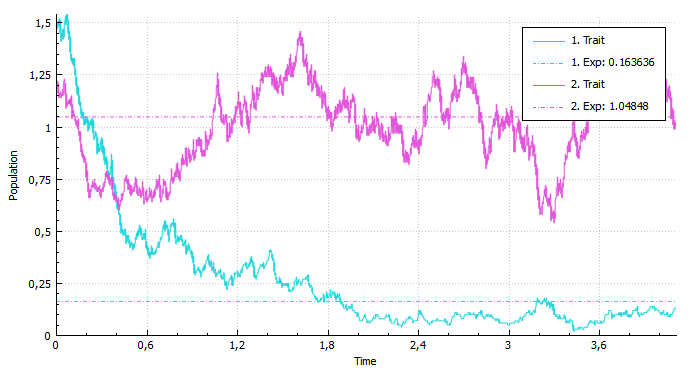
\includegraphics[width=1\linewidth]{./Pictures/LPANormalisierungK100}%
		\\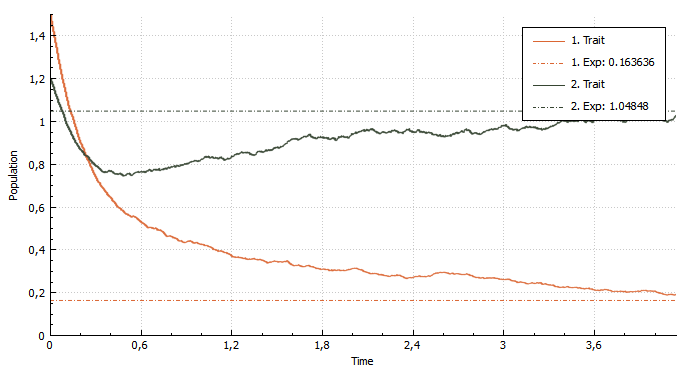
\includegraphics[width=1\linewidth]{./Pictures/LPANormalisierungK10000}%
		\end{figure}
	\end{minipage}
	\begin{minipage}{0.49\textwidth}
		Bsp. einer LPA-Normalisierung mit $ K = 100 \text{ und } K = 10000 $:
		\begin{itemize}
			\item Flacherer Verlauf der zeitlichen Entwicklung.\pause
			\item Einzelne Ereignisse lassen sich nicht mehr nachvollziehen.\pause
			\item Mit wachsendem K wird der Prozess zunehmend deterministisch und weicht immer weniger von anderen Simulationen ab.
		\end{itemize}
	\begin{center}
	\end{center}
	\end{minipage}\\
\end{frame}

\begin{frame}{Konvergenz}
	Solch ein deterministisches System erf"ullt (beispielhaft f"ur zwei Merkmale):
	\begin{align*}
	\dot{n}(x) = n(x) \left( b(x) - d(x) - c(x,x) n(x) - c(x,y) n(y) \right)\\
	\dot{n}(y) = n(y) \left( b(y) - d(y) - c(y,y) n(y) - c(y,x) n(x) \right)\\
	n_0(y) = n_{0,y}, n_0(x) = n_{0,x}
	\end{align*}\pause
	Mit Theorem 2.1 aus Ethier und Kurtz; Markov Processes: characterization and convergence - Kapitel 11 erhalten wir die Konvergenz $ \nu_t^K \xrightarrow{K\to \infty} n_t $.
\end{frame}

\subsection{Gleichgewicht}
\begin{frame}
	\frametitle{Gleichgewicht}
	In einem stabilen Zustand ändert sich die Populationsgröße nicht mehr:\smallskip\\\pause
	\begin{minipage}{0.49\textwidth}
	$ \rhd $ Für monomorphe Population:
		\begin{align*}
		0 	&= (b(x) - d(x) - \bar{n}c(x,x))\bar{n}\\
		\bar{n}_x &= \frac{\left[ b(x)-d(x) \right]_+}{c(x,x)}
		\end{align*}\pause
	\end{minipage}
	\begin{minipage}{0.49\textwidth}
		\begin{figure}[H]
			\centering
			\includegraphics[width=1\linewidth]<2->{./Pictures/BigKInstance_Equillibrium}
		\end{figure}
	\end{minipage}
	\\
	$ \rhd $ Für dimorphe Population:
	\[ n_x = \frac{(b(x) - d(x))c(y,y)-(b(y)-d(y))c(x,y)}{c(y,y)c(x,x) - c(y,x)c(x,y)} \]
	$ \Rightarrow (n_x, n_y), (\bar{n}_x, 0), (0, \bar{n}_y) \text{ und } (0,0) $ sind mögliche stabile Zustände der dimorphen Population.
%	oder $ (\bar{n}_x, 0)$, $ (0, \bar{n}_y)$ bzw. $ (0,0) $
\end{frame}

\subsection{Fitness}
\begin{frame}
	\frametitle{Fitness-Funktion}
	\begin{minipage}{0.49\textwidth}
	Wann wird welches Gleichgewicht angenommen?\pause
	\[ f(x,y) = b(x) - d(x) - c(x,y)\bar{n}_y \]\pause
	\end{minipage}
	\begin{minipage}{0.49\textwidth}
	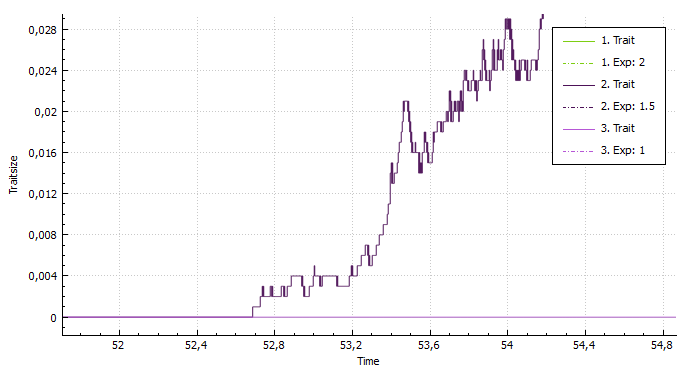
\includegraphics[width=1\linewidth]{./Pictures/Mutation_posFitness}
	\end{minipage}	
	\begin{itemize}
		\item Sie gibt an wie gut sich ein Merkmal durchsetzten kann.\pause
		\item Asymptotische Wachstumsrate von y, wenn x im Zustand $ \bar{n}_x $ ist und y nur wenige Individuen hat.\pause
		\item Ermöglicht Aussagen über die Überlebenswahrscheinlichkeit einer Mutation.\pause
		\item Ermöglicht Aussagen über die angenommenen stabilen Zustände.\pause
	\end{itemize}
	Da wir nur eine Mutation zu den Nachbarn berücksichtigen, ist unsere Fitness Matrix eine Bandmatrix.
\end{frame}

\subsection{TSS-Prozesse}
\begin{frame}{Was ist ein TSS-Prozess?}
	\begin{itemize}
		\item Wie bei LPA-Normalisierung ergeben sich TSS-Prozesse als Grenzprozesse von BPDL-Prozessen.
		\pause
		\item Jedoch mit wachsendem K schrumpft $ \mu $ mit der Ordnung:
		\[ \frac{1}{e^{VK}} << \mu_K << \frac{1}{K log(K)} \]
		\pause
		\item Mit skalierter Zeit, wird die Dauer der Verdr"angung infinitesimal klein.
		\pause
		\item Spr"unge zwischen monomorphen Zust"anden, falls stets $ f(x,y) < 0 \text{ \& } f(y,x) > 0 $. H"ochstens zwei Merkmale vereinfachen die Analyse des Prozesses sehr.
	\end{itemize}
\end{frame}

\begin{frame}{TSS-Approximation}
	F"ur die Simulation w"urde das insbesondere bedeuten dass viele Spr"unge im Gleichgewicht zu erwarten sind.\pause
	Eine Simulation würde bisher so aussehen (K = 1000):
	\begin{figure}[H]
		\centering
		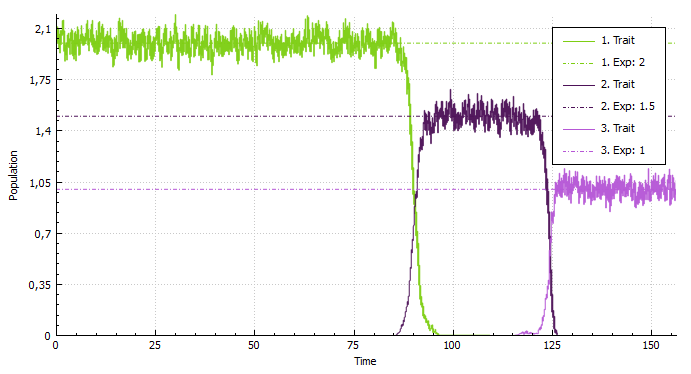
\includegraphics[width=0.8\linewidth]{./Pictures/TSS2_pure_small}
		\caption[TSS Approximation wechselnder Dominanz]{TSS-Approximation mit: K = 1000 und $ 4 \cdot 10^6 $ Sprüngen}
	\end{figure}
\end{frame}

\section{Simulation}
\begin{frame}{Was und wie wird simuliert?}
	\begin{itemize}
		\item Ein Sprung des BPDL-Prozesses (evolution step).
		\item Implementation: Sorgf"altige Trennung der Aufgaben.\\
			Pseudocode: Gesamter Arbeitsablauf.
		\item "Ubersichtlich und mit transparentem Ablauf.\pause
	\end{itemize}
	Folgend ist ein Diagramm zur kompakten Darstellung der Implementierung und anschlie"send der Pseudocode in zwei Teilen.
\end{frame}

\subsection{Implemen\- tierung}
\begin{frame}
	\begin{figure}[H]
		\centering
		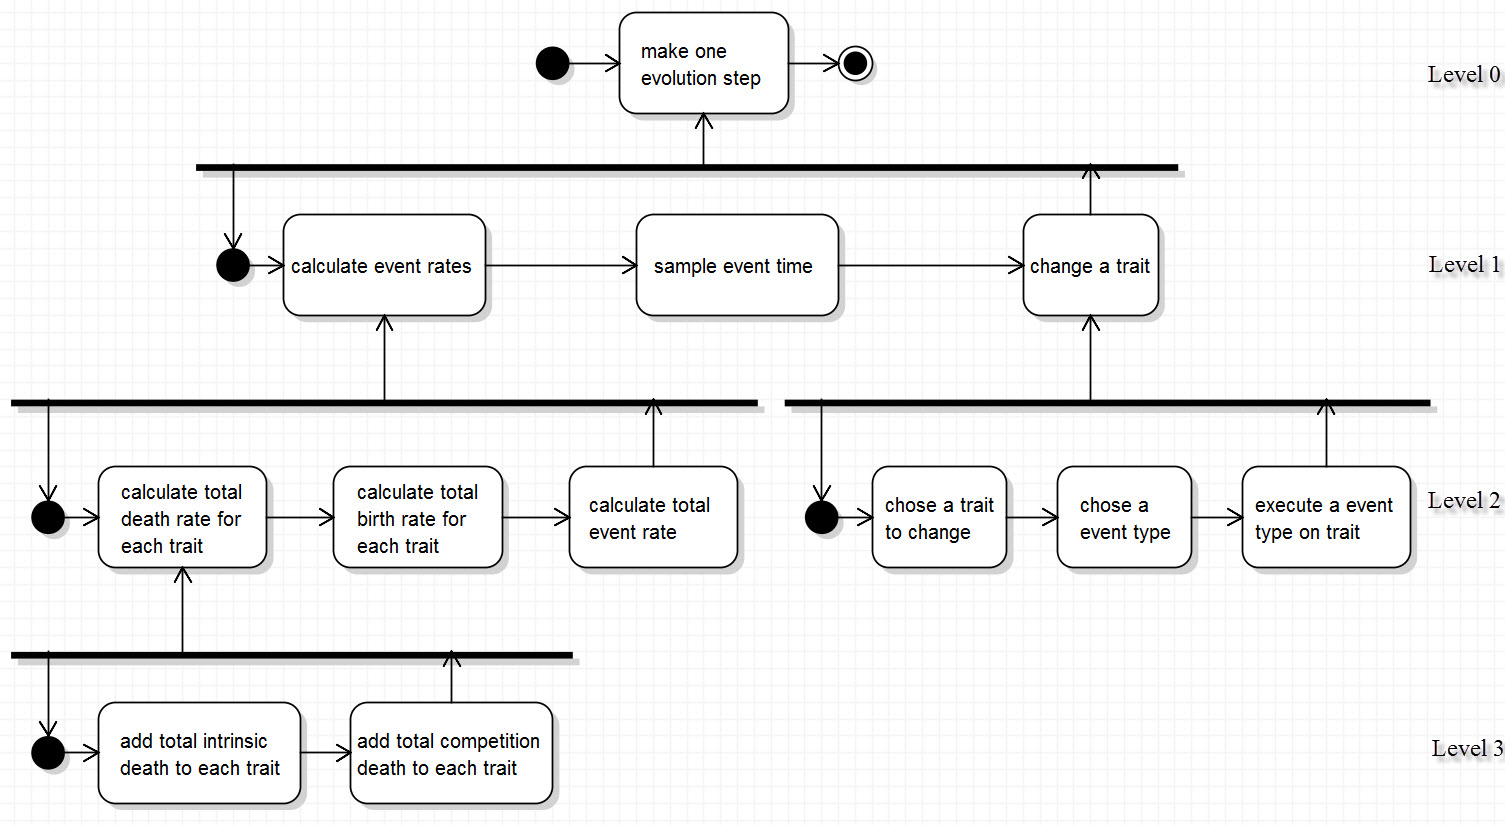
\includegraphics[width=1\linewidth]{../UMLs/PseudoCodeForBThesis}
		\caption{Diagramm mit Funktionsaufrufen und ihren Tiefenebenen}
	\end{figure}
\end{frame}

\subsection{Pseudocode}
\begin{frame}
	\begin{figure}[H]
		\centering
		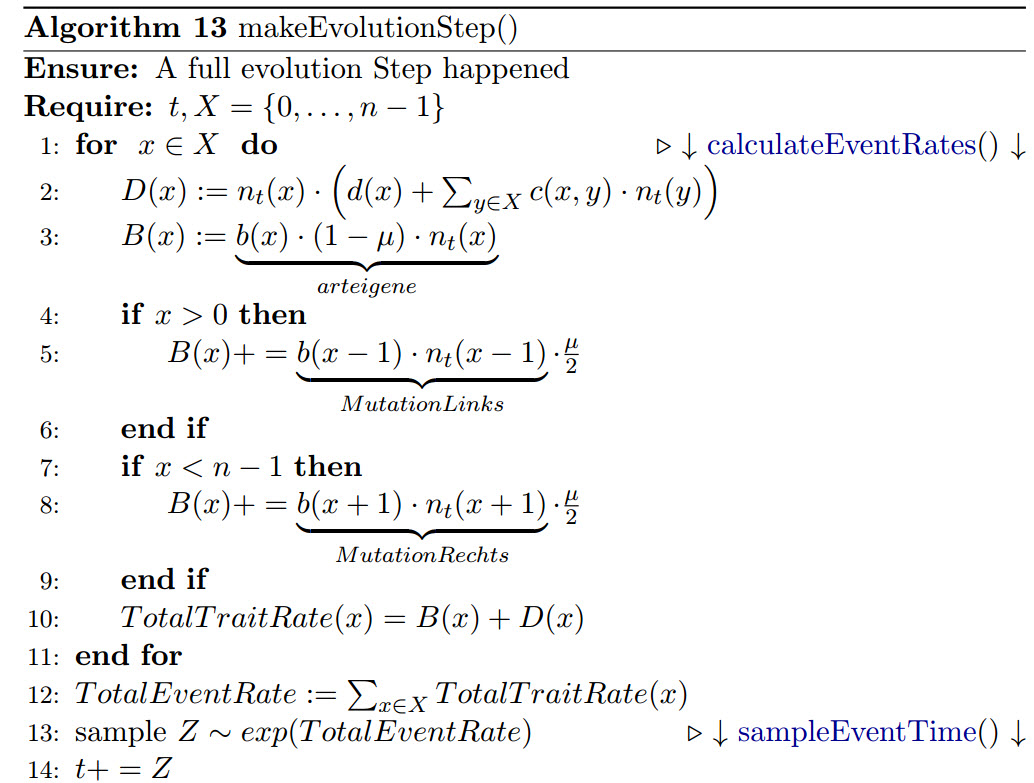
\includegraphics[width=1\linewidth]{./Pictures/Alg1}
	\end{figure}
\end{frame}
\begin{frame}
	\begin{figure}[H]
		\centering
		\includegraphics[width=1\linewidth]<1,3->{./Pictures/Alg2}
		\includegraphics[width=1\linewidth]<2>{./Pictures/SelectTrait}		
	\end{figure}
\end{frame}

\subsection{Optimierung}
\begin{frame}{Viele Merkmale?}
Bisher ist der Aufwand linear in der Anzahl der Spr"unge, doch quadratisch in Abh"angigkeit der Merkmale.\pause Daf"ur wurde in der BA eine Optimierung vorgestellt:
	\begin{itemize}
		\item Gr"o"ster zeitlicher Aufwand in Berechnung der Raten (Ursache f"ur Aufwand). Idee: Vermeidung der Neuberechnung.\pause
		\item Anpassung der Raten nach eintreten eines Ereignisses! Schritt beginn mit Ausf"uhrung der aktuellen Raten.
	\end{itemize}
\end{frame}

\begin{frame}{Viele Spr"unge und Normalisierung?}
Gerade mit gro"sem K werden viele Spr"unge notwendig. Diese werden schnell den Speicher "uberfluten.\pause\bigskip\\
Daf"ur habe ich zwei L"osungen entwickelt und implementiert:\\
$ \rhd $ "{}erweiterte Spr"unge"{} - Speicherung von Messpunkten\\
$ \rhd $ "{}Storage"{} - Eine ausgelagerte tempor"are Datei\bigskip\\\pause
Wo wird eigentlich die Normalisierung angewendet?\\\pause
$ \rhd $ \textcolor{blue}{Kein Einfluss auf den evolution"aren Mechanismus}.\\
$ \rhd $ Beim Einlesen und bei Zugriffen.\\
\end{frame}

\section{Programm}
\begin{frame}
	\frametitle{Flexibilität}
	Um Flexibilität aufrecht zu erhalten werden die Arbeitsbereiche im Code getrennt gehalten.\\
	\pause
	Grund der Idee:
	\begin{itemize}
		\item Möglichst viel Unabhängigkeit
		\pause
		\item verhindert "{}Coderot"{} - faulen Code
		\pause
		\item steigende Komplexität führt nicht zu undefiniertem Verhalten
		\pause
		\item "{}Single Responsibility Principle"{}. Es darf nur einen Grund zur "Anderung geben.
		\pause
		\item 
	\end{itemize}
\end{frame}
\begin{frame}
	\frametitle{Arbeitsmodule}
	Die Architektur besteht aus 3 Modulen
	\pause
	\begin{figure}[H]
		\centering
		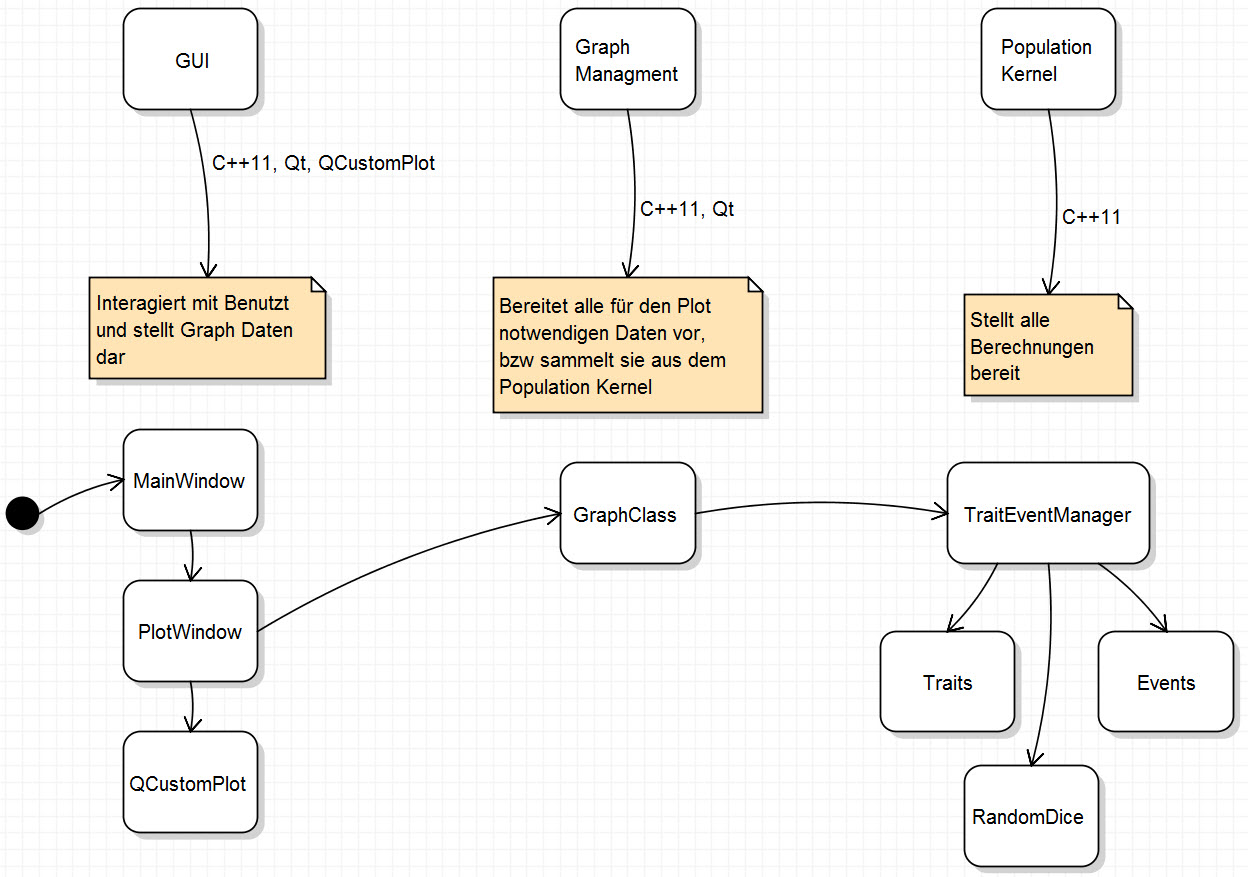
\includegraphics[width=0.8\linewidth]{./Pictures/Bild_Module}
		\caption[Module]{Arbeitsmodule und Klassenabhängigkeiten}
		\label{Module und Klassen}
	\end{figure}
\end{frame}

\subsection{Parameter}
\begin{frame}{Start}
	\begin{minipage}{1\textwidth}
		\begin{figure}[H]
			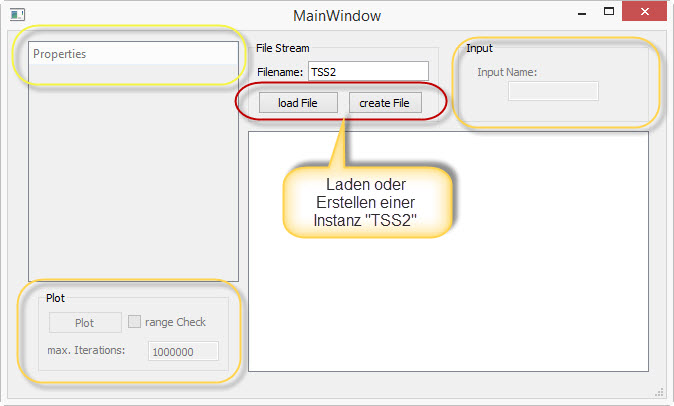
\includegraphics[width=1\linewidth]{./Pictures/MainWindow_Start}
			\caption[Startwindow]{MainWindow nach dem Start}
		\end{figure}
	\end{minipage}
\end{frame}
\begin{frame}{Lade Parameter}
	\begin{minipage}{0.45\textwidth}
		\begin{figure}[H]
			\centering
			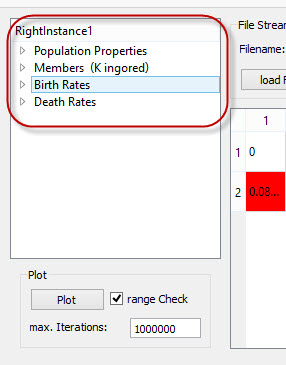
\includegraphics[width=1\linewidth]{./Pictures/MainWindow_ParameterBaum_zu}
			\caption[MainWindow_Parameter]{Baumstruktur - geschlossen}
			\label{Baumstruktur_geschlossen}
		\end{figure}
	\end{minipage} $ \quad $
	\begin{minipage}{0.45\textwidth}
		\begin{figure}[H]
			\centering
			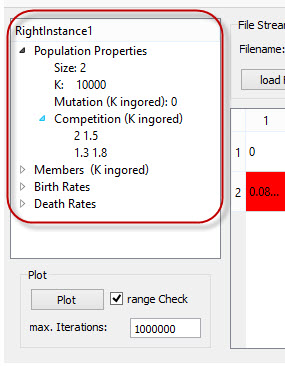
\includegraphics[width=1\linewidth]{./Pictures/MainWindow_ParameterBaum_offen}
			\caption[MainWindow_Parameter]{Verzweigte Baumstruktur - geöffnet}
			\label{Baumstruktur_offen}
		\end{figure}
	\end{minipage}
\end{frame}
\begin{frame}{Erstelle Parameter}
	\begin{figure}[H]
		\centering
		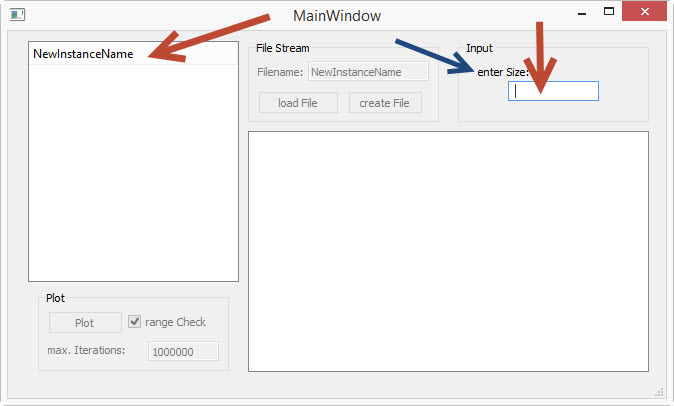
\includegraphics[width=1\linewidth]{./Pictures/MainWindow_createFile}\bigskip\\
		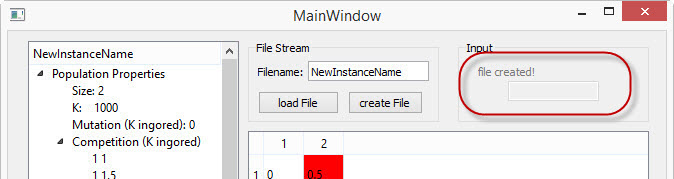
\includegraphics[width=1\linewidth]{./Pictures/MainWindow_FileCreated}
	\end{figure}
\end{frame}

\subsection{Darstellung}
\begin{frame}{Graphische Darstellung}
	An die graphische Darstellung wurden folgende Anforderungen gesetzt:
	\begin{itemize}
		\item Man soll den zeitlichen Verlauf der Populationsgrößen beobachten \- können.
		\item Um die Prozesse besser analysieren zu können, soll es möglich sein, Stellen des Graphen näher betrachten zu können (zoom).
		\item Um Simulationen vergleichen zu können, sollen außerdem Ausschnitte als Bilder gespeichert werden können.
		\item Und natürlich soll das Programm bei der Berechnung nicht abstürzen.
	\end{itemize}
\end{frame}

\begin{frame}{Multithreading}
	Der letzte Punkt ist bei der Ereignisgesteuerten Programmierung tats"achlich eine nicht triviale H"urde. Daf"ur m"ussen Threads verwendet werden. Dabei muss auf einige Punkte geachtet werden, z.B.:\smallskip\\
	\begin{minipage}{0.49\textwidth}
	\begin{itemize}
		\item Konfliktfreies Arbeiten (nicht Ereignisgesteuert).
		\item Race Conditions.
		\item Deadlocks (Endlos warteschleife).
	\end{itemize}
	\end{minipage}
	\begin{minipage}{0.49\textwidth}
	\begin{figure}[H]
		
\includegraphics[width=1\linewidth]{./Pictures/KeineRueckmeldung}
	\end{figure}
	\end{minipage}\\\smallskip
	Die L"osungen sind sogar bei erkanntem Problem nicht immer einfach zu finden. Bsp. Philosophenproblem.
\end{frame}

\begin{frame}{Plot}
	In blau sieht man, dass das Programm durch Übereinanderlegen während der Berechnung weiterhin ansprechbar ist statt keine Rückmeldung zu liefern.
	\begin{figure}[H]
		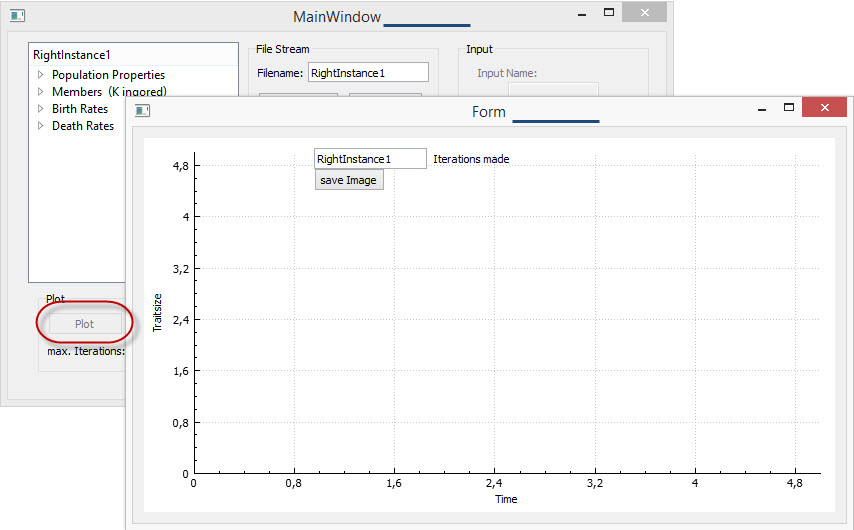
\includegraphics[width=0.75\linewidth]{./Pictures/PlotWindow_start}
		\caption[PlotWindow_start]{Start des PlotWindow}
	\end{figure}
\end{frame}

\begin{frame}{Plot}
	Nach der Berechnung, werden die Punkte verbunden. Das Ergebnis sieht folgenderma"sen aus:
	\begin{figure}[H]
		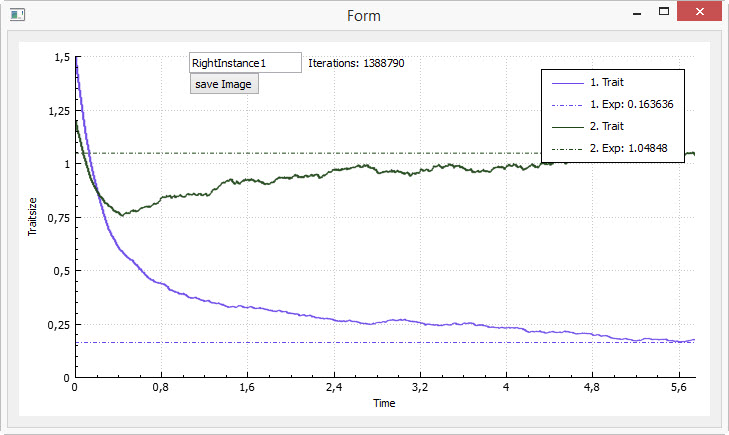
\includegraphics[width=0.85\linewidth]{./Pictures/PlotWindow_smallBPDL}
		\caption[PlotWindow]{PlotWindow mit Dimorpher Population}
	\end{figure}
\end{frame}

\begin{frame}{Optionen}
	Was bietet die graphische Darstellung?\smallskip\\
	\begin{minipage}{0.42\textwidth}
	\begin{itemize}
		\item zeitliche Entwicklung.
		\item stabile Zust"ande.
		\item ben"otigte Spr"unge.
		\item Legende der Graphen.
		\item speichern des Bildes.
	\end{itemize}
	\end{minipage}
	\begin{minipage}{0.56\textwidth}
	\begin{figure}[H]
		\centering
		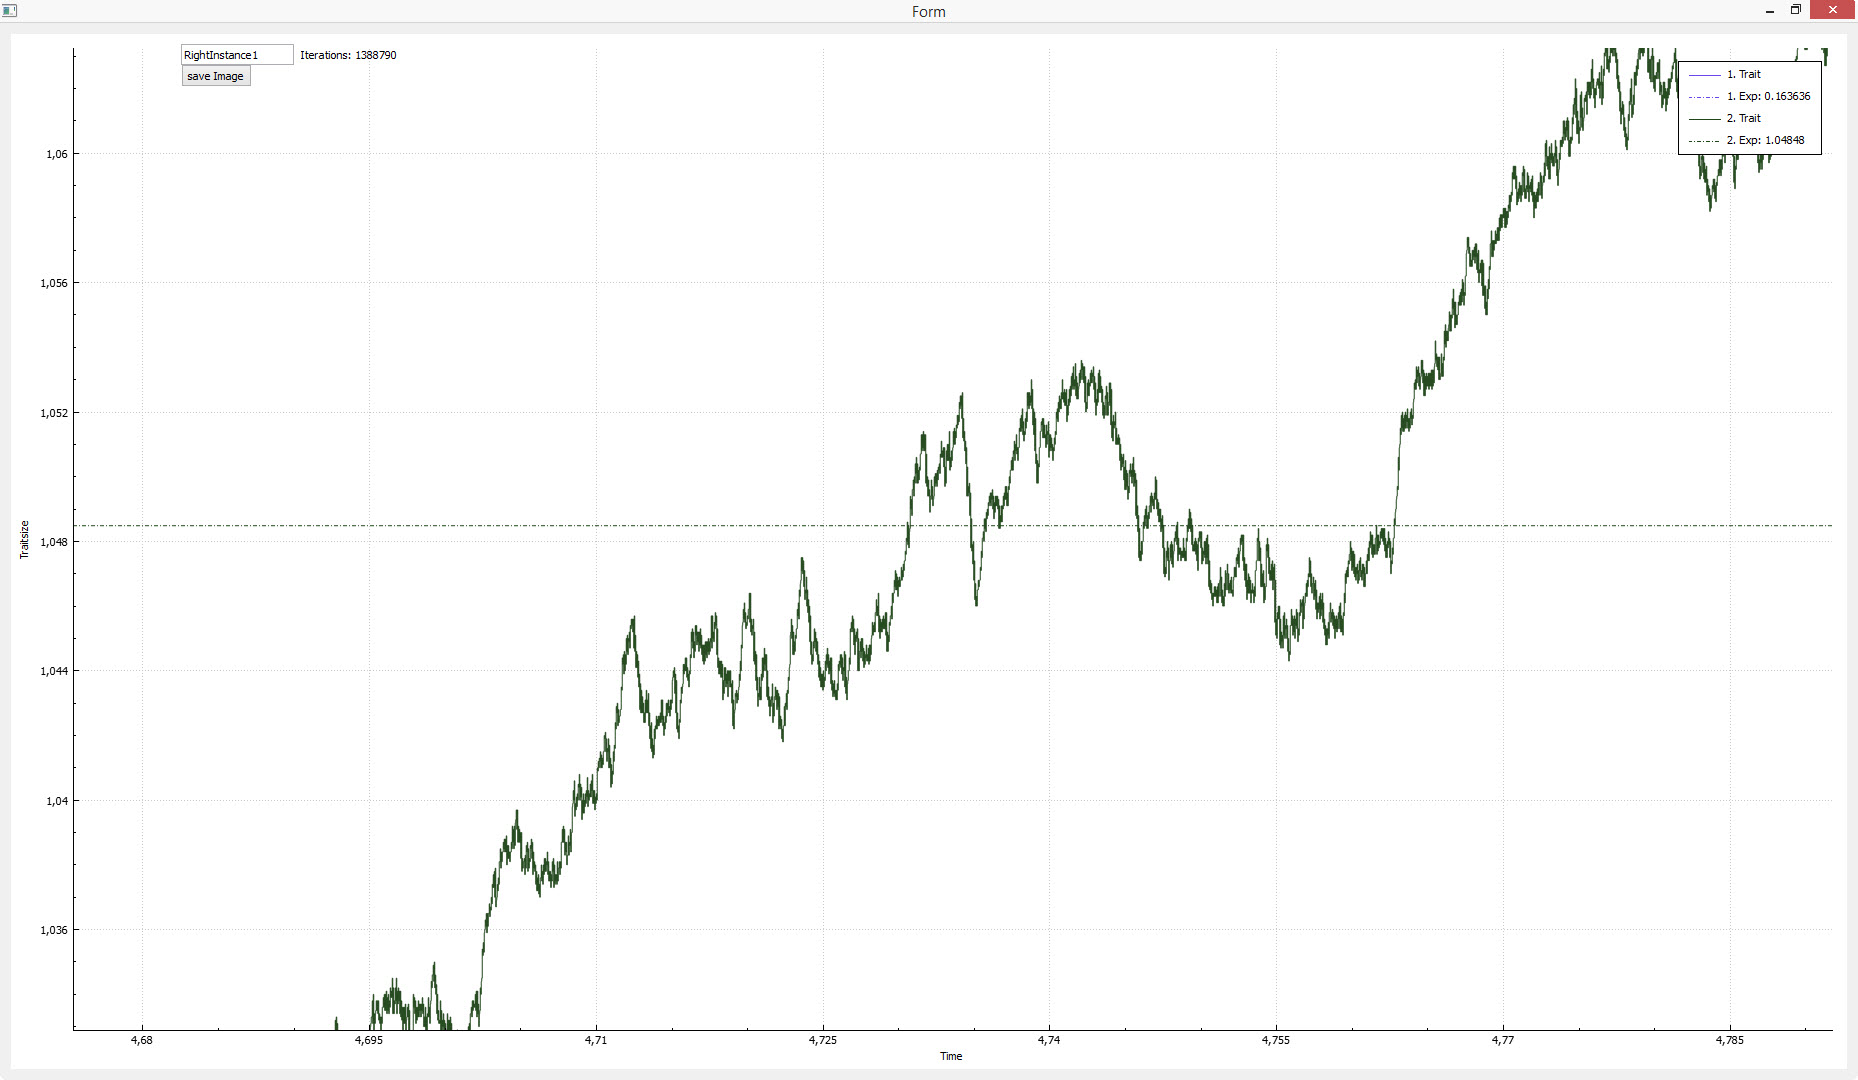
\includegraphics[width=0.9\linewidth]{./Pictures/PlotWindow_zoomedBPDLmaximized}
	\end{figure}
	\end{minipage}\smallskip\\
	Des weiteren lasst sich das Bild manipulieren:
	\begin{itemize}
		\item Zoom mit automatisch anpassbarem Messgitter.
		\item Bewegung durch Ziehbewegungen.
		\item freie Skalierbarkeit des Bildes.
	\end{itemize}
\end{frame}

\section{Verhaltens- tests}
\begin{frame}{Testgetriebene Entwicklung}
Die Korrektheit der Implementation ist mit zunehmender Komplexität des Codes schwerer zu prüfen (ganz besonders bei Zufallsbedingten Simulationen). Deswegen habe ich mich zu Beginn der BA mit TDD besch"aftigt.\\
Was ist TDD und was tut ein Unit Test?
\begin{itemize}
	\item eine Funktion die erwartetes Verhalten mit der Implementierung vergleicht.
	\item gew"ahrleisten Bedingungen um "Anderungen und Funktionalit"at so souver"an wie m"oglich zu gestalten.
\end{itemize}
Aber warum sollten solche Tests Korrektheit des Programms gew"ahrleisten?
\end{frame}

\begin{frame}{Korrektheit}
Die Korrektheit eines Programmkerns nachzuweisen kann sich als schwierig
herausstellen, weil man die Korrektheit nicht für eine spezifische Instanz,
sondern flexibel für alle nachweisen möchte. Doch ist es nicht notwendig
die Flexibilität des Programms zu testen, wenn man stattdessen versucht,
die Korrektheit jedes Arbeitsschrittes zu prüfen. Ein Arbeitsschritt erhebt
in unserem Fall keinen Anspruch auf Komplexität. Tatsächlich sind unsere
Arbeitsschritte alle möglichst einfach und erfüllen nur eine Aufgabe. D.h.
die Korrektheit der Arbeitsschritte zu verifizieren lässt sich denkbar einfach mit einem Test abdecken.
\end{frame}

\section{TSS}
\begin{frame}{Invasion}

\end{frame}

\begin{frame}{Phasen einer Invasion}

\end{frame}

\begin{frame}{Optimierung}
Inhalt...
\end{frame}

\begin{frame}{Implementierung}
Inhalt...
\end{frame}

\end{document}
% ä Ä ö Ö ü Ü